\documentclass[letter,11pt]{article}

\usepackage[spanish,es-nodecimaldot]{babel}
\usepackage[utf8]{inputenc}

\usepackage{lmodern}
\usepackage[T1]{fontenc}
\usepackage{textcomp}

\usepackage{framed}
\usepackage[svgnames]{xcolor}
\colorlet{shadecolor}{Gainsboro!50}

\usepackage{enumitem}
\usepackage{graphicx}
\usepackage{pstricks}

\usepackage{anysize}
\marginsize{3cm}{2cm}{2cm}{3cm}

\usepackage{siunitx}
\usepackage{amsmath}
\usepackage{array}
\usepackage{alltt}

\usepackage{fancyhdr}
\usepackage{lastpage}
\pagestyle{fancy}
\fancyhf{}
\fancyhead[LE,RO]{Física Básica III}
\fancyfoot[CO,CE]{\thepage\ de \pageref{LastPage}}

\special{papersize=215.9mm,279.4mm}

\usepackage[
    pdfauthor={Carlos Eduardo Caballero Burgoa},%
    pdftitle={Física Básica III},%
    pdfsubject={Tarea},%
    colorlinks,%
    citecolor=black,%
    filecolor=black,%
    linkcolor=black,%
    urlcolor=black,
    breaklinks]{hyperref}
\usepackage{breakurl}

\newcommand{\blankpage}{
\newpage
\thispagestyle{empty}
\mbox{}
\newpage
}

\renewcommand{\arraystretch}{1.2}

\begin{document}

\begin{center}
    {\Large \bf{\underline{Tarea}}}
\end{center}

\textbf{\underline{Capacitancia en un condensador cilíndrico}:} \\

\begin{figure}[!h]
\centering
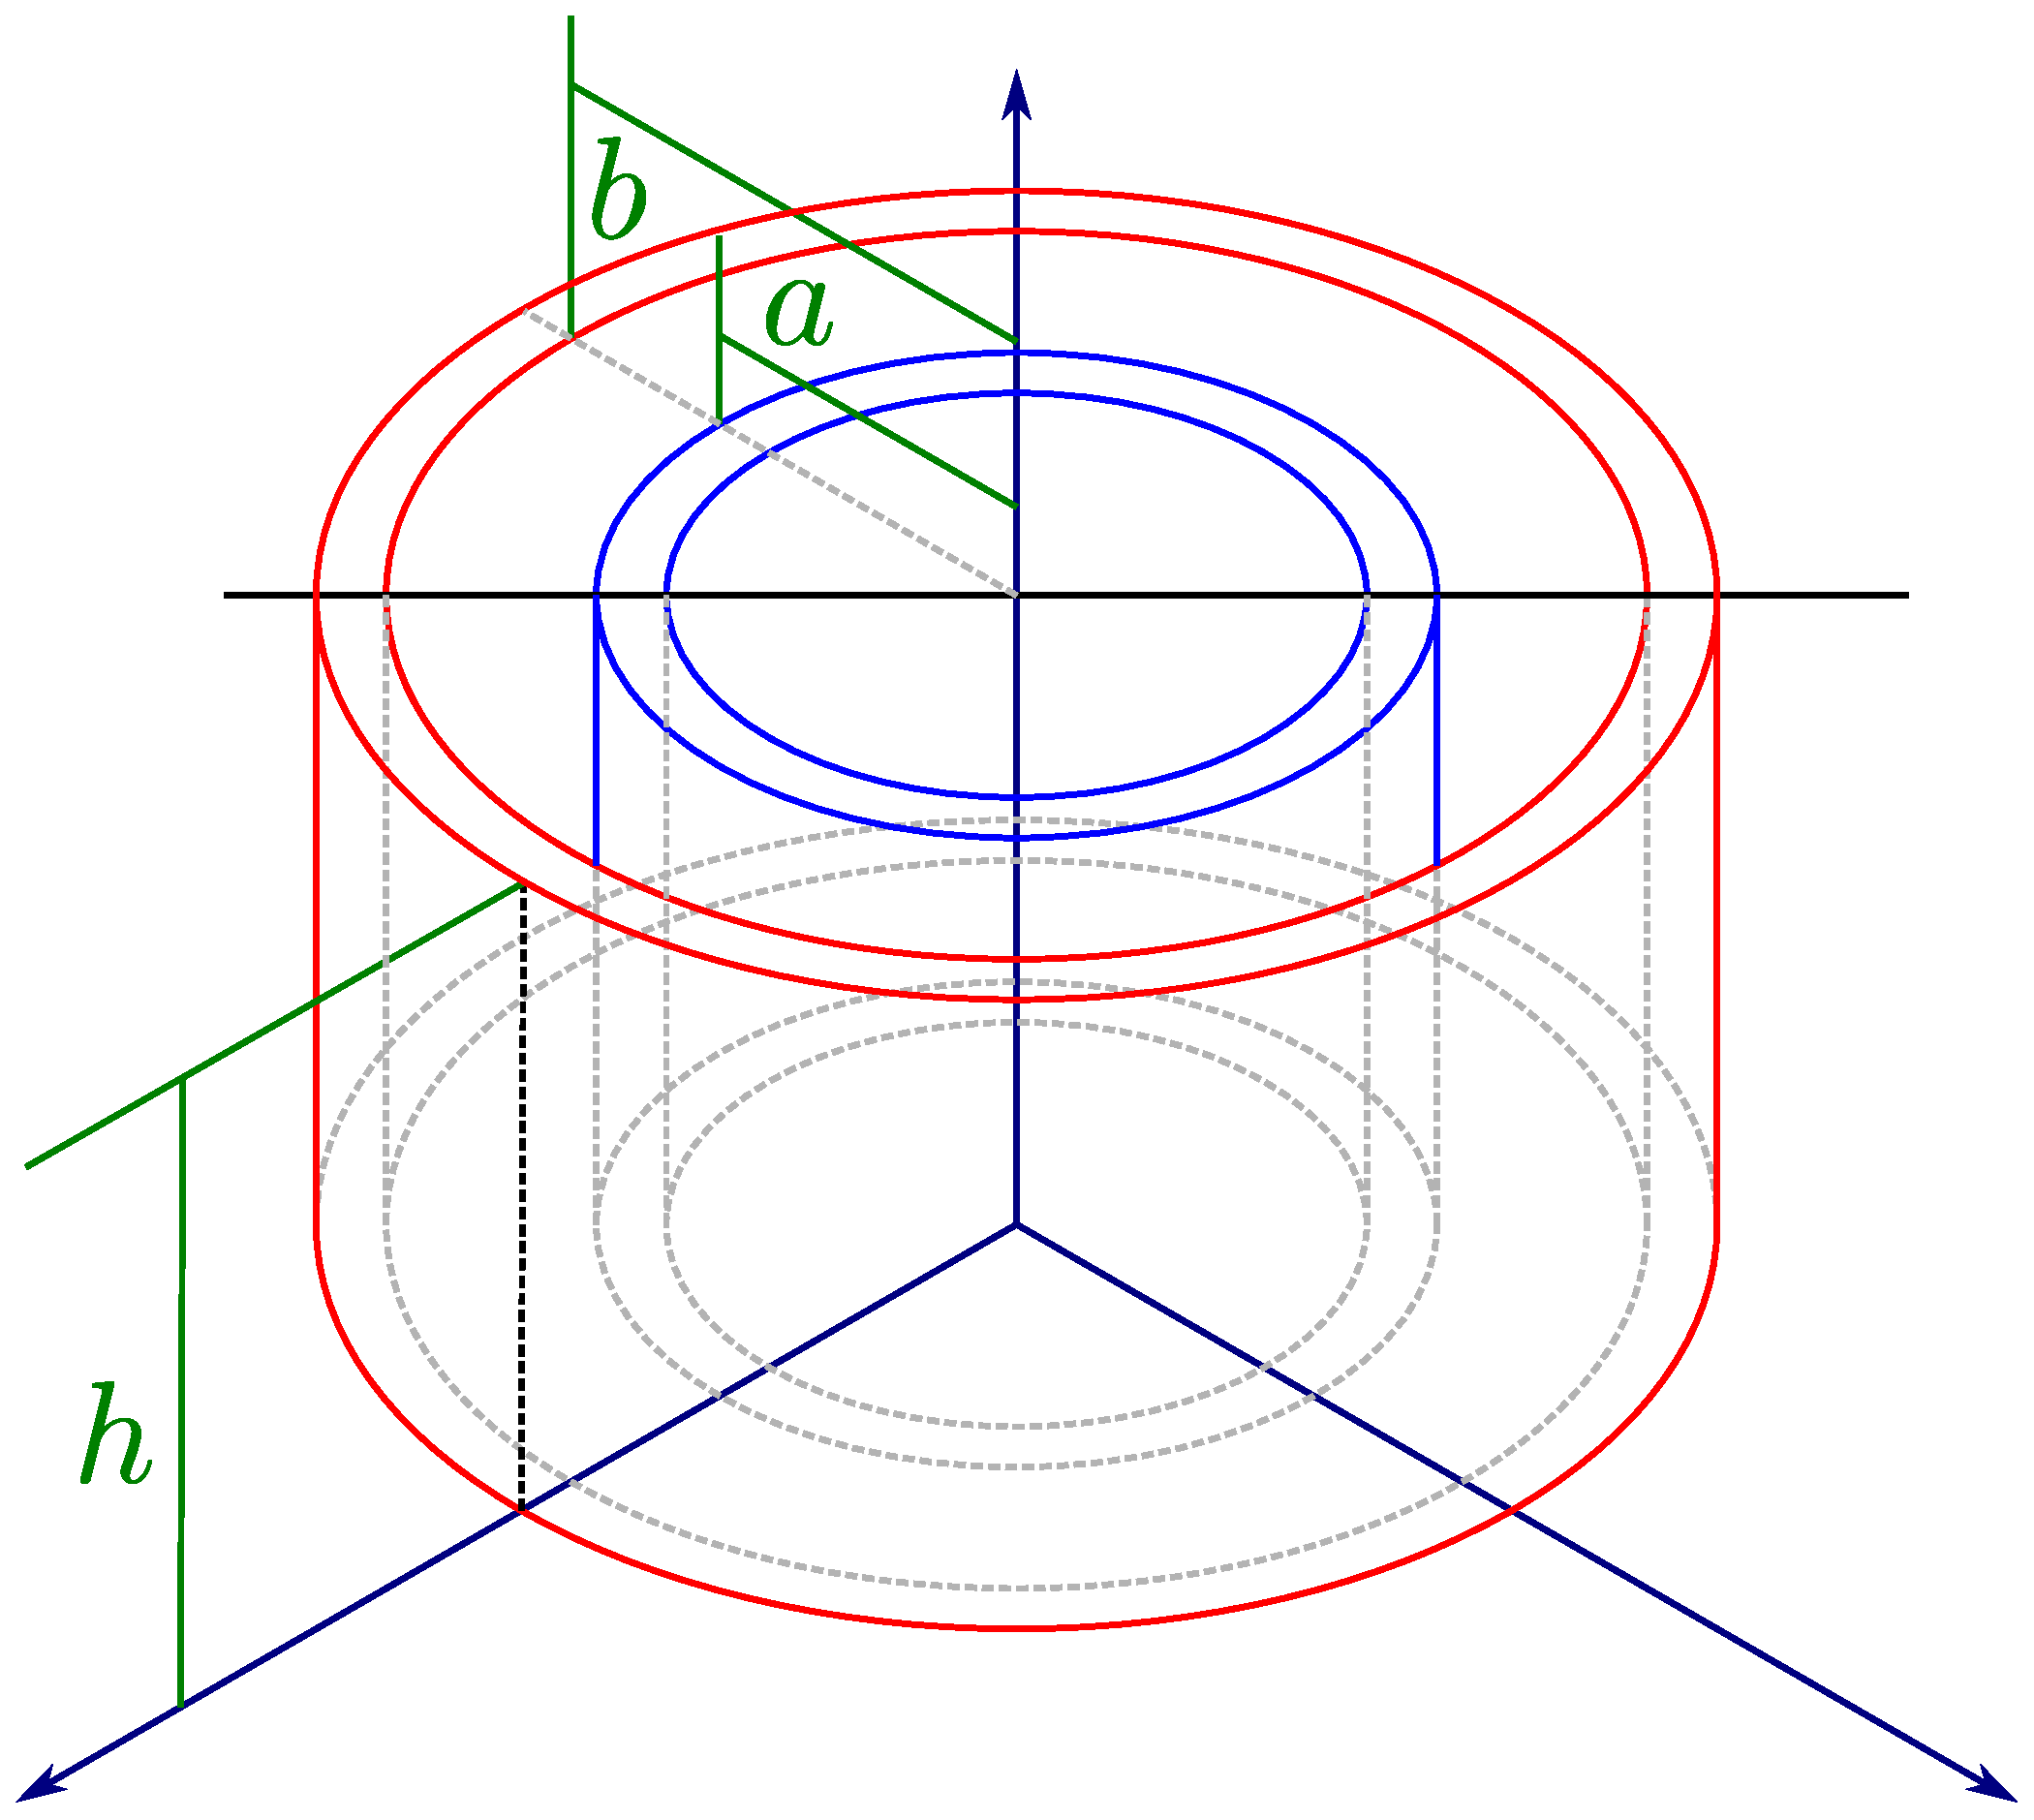
\includegraphics[scale=0.15]{resources/f1.eps}
\end{figure}
\vspace{0.5cm}

Usando una superficie \emph{gaussiana} sobre el capacitor para obtener el campo
eléctrico:

\begin{equation*}
    \oint\vec{E}\cdot d\vec{A}=\frac{Q_{enc}}{\epsilon_0}
\end{equation*}
\begin{equation*}
    E\,(2\pi r h)=\frac{Q}{\epsilon_0}
\end{equation*}
\begin{equation*}
    E=\frac{Q}{\epsilon_0}\frac{1}{2\pi r h}
     =\frac{Q}{2\pi\epsilon_0 r h}
\end{equation*}
\begin{equation*}
    \vec{E}=\frac{Q}{2\pi\epsilon_0 r h}\hat{u}_r
\end{equation*}
\vspace{0.5cm}

Calculando la diferencia de potencial eléctrico:

\begin{equation*}
    \hat{E}=-\nabla\varphi
\end{equation*}
\begin{equation*}
    \frac{Q}{2\pi\epsilon_0 r h}\hat{u}_r=-\frac{d\varphi}{dr}\hat{u}_r
\end{equation*}
\begin{equation*}
    \frac{Q}{2\pi\epsilon_0 r h}dr=-d\varphi
\end{equation*}
\begin{equation*}
    \frac{Q}{2\pi\epsilon_0 h}\int_a^b\frac{dr}{r}
    =-\int_{\varphi^+}^{\varphi^-}d\varphi
\end{equation*}
\begin{equation*}
    V=\frac{Q}{2\pi\epsilon_0 h}(ln(r)\Biggr|_a^b)
     =\frac{Q}{2\pi\epsilon_0 h}(ln(b)-ln(a))
     =\frac{Q}{2\pi\epsilon_0 h}ln\left(\frac{b}{a}\right)
\end{equation*}
\vspace{0.5cm}

Considerando la definición de capacitancia $Q=CV$:

\begin{equation*}
    C=\frac{Q}{V}
     =Q\,\frac{2\pi\epsilon_0 h}{Q\,ln(\frac{b}{a})}
     =\frac{2\pi\epsilon_0 h}{ln(\frac{b}{a})}
\end{equation*}
\vspace{0.75cm}

\textbf{\underline{Capacitancia en un condensador esférico}:} \\

\begin{figure}[!h]
\centering
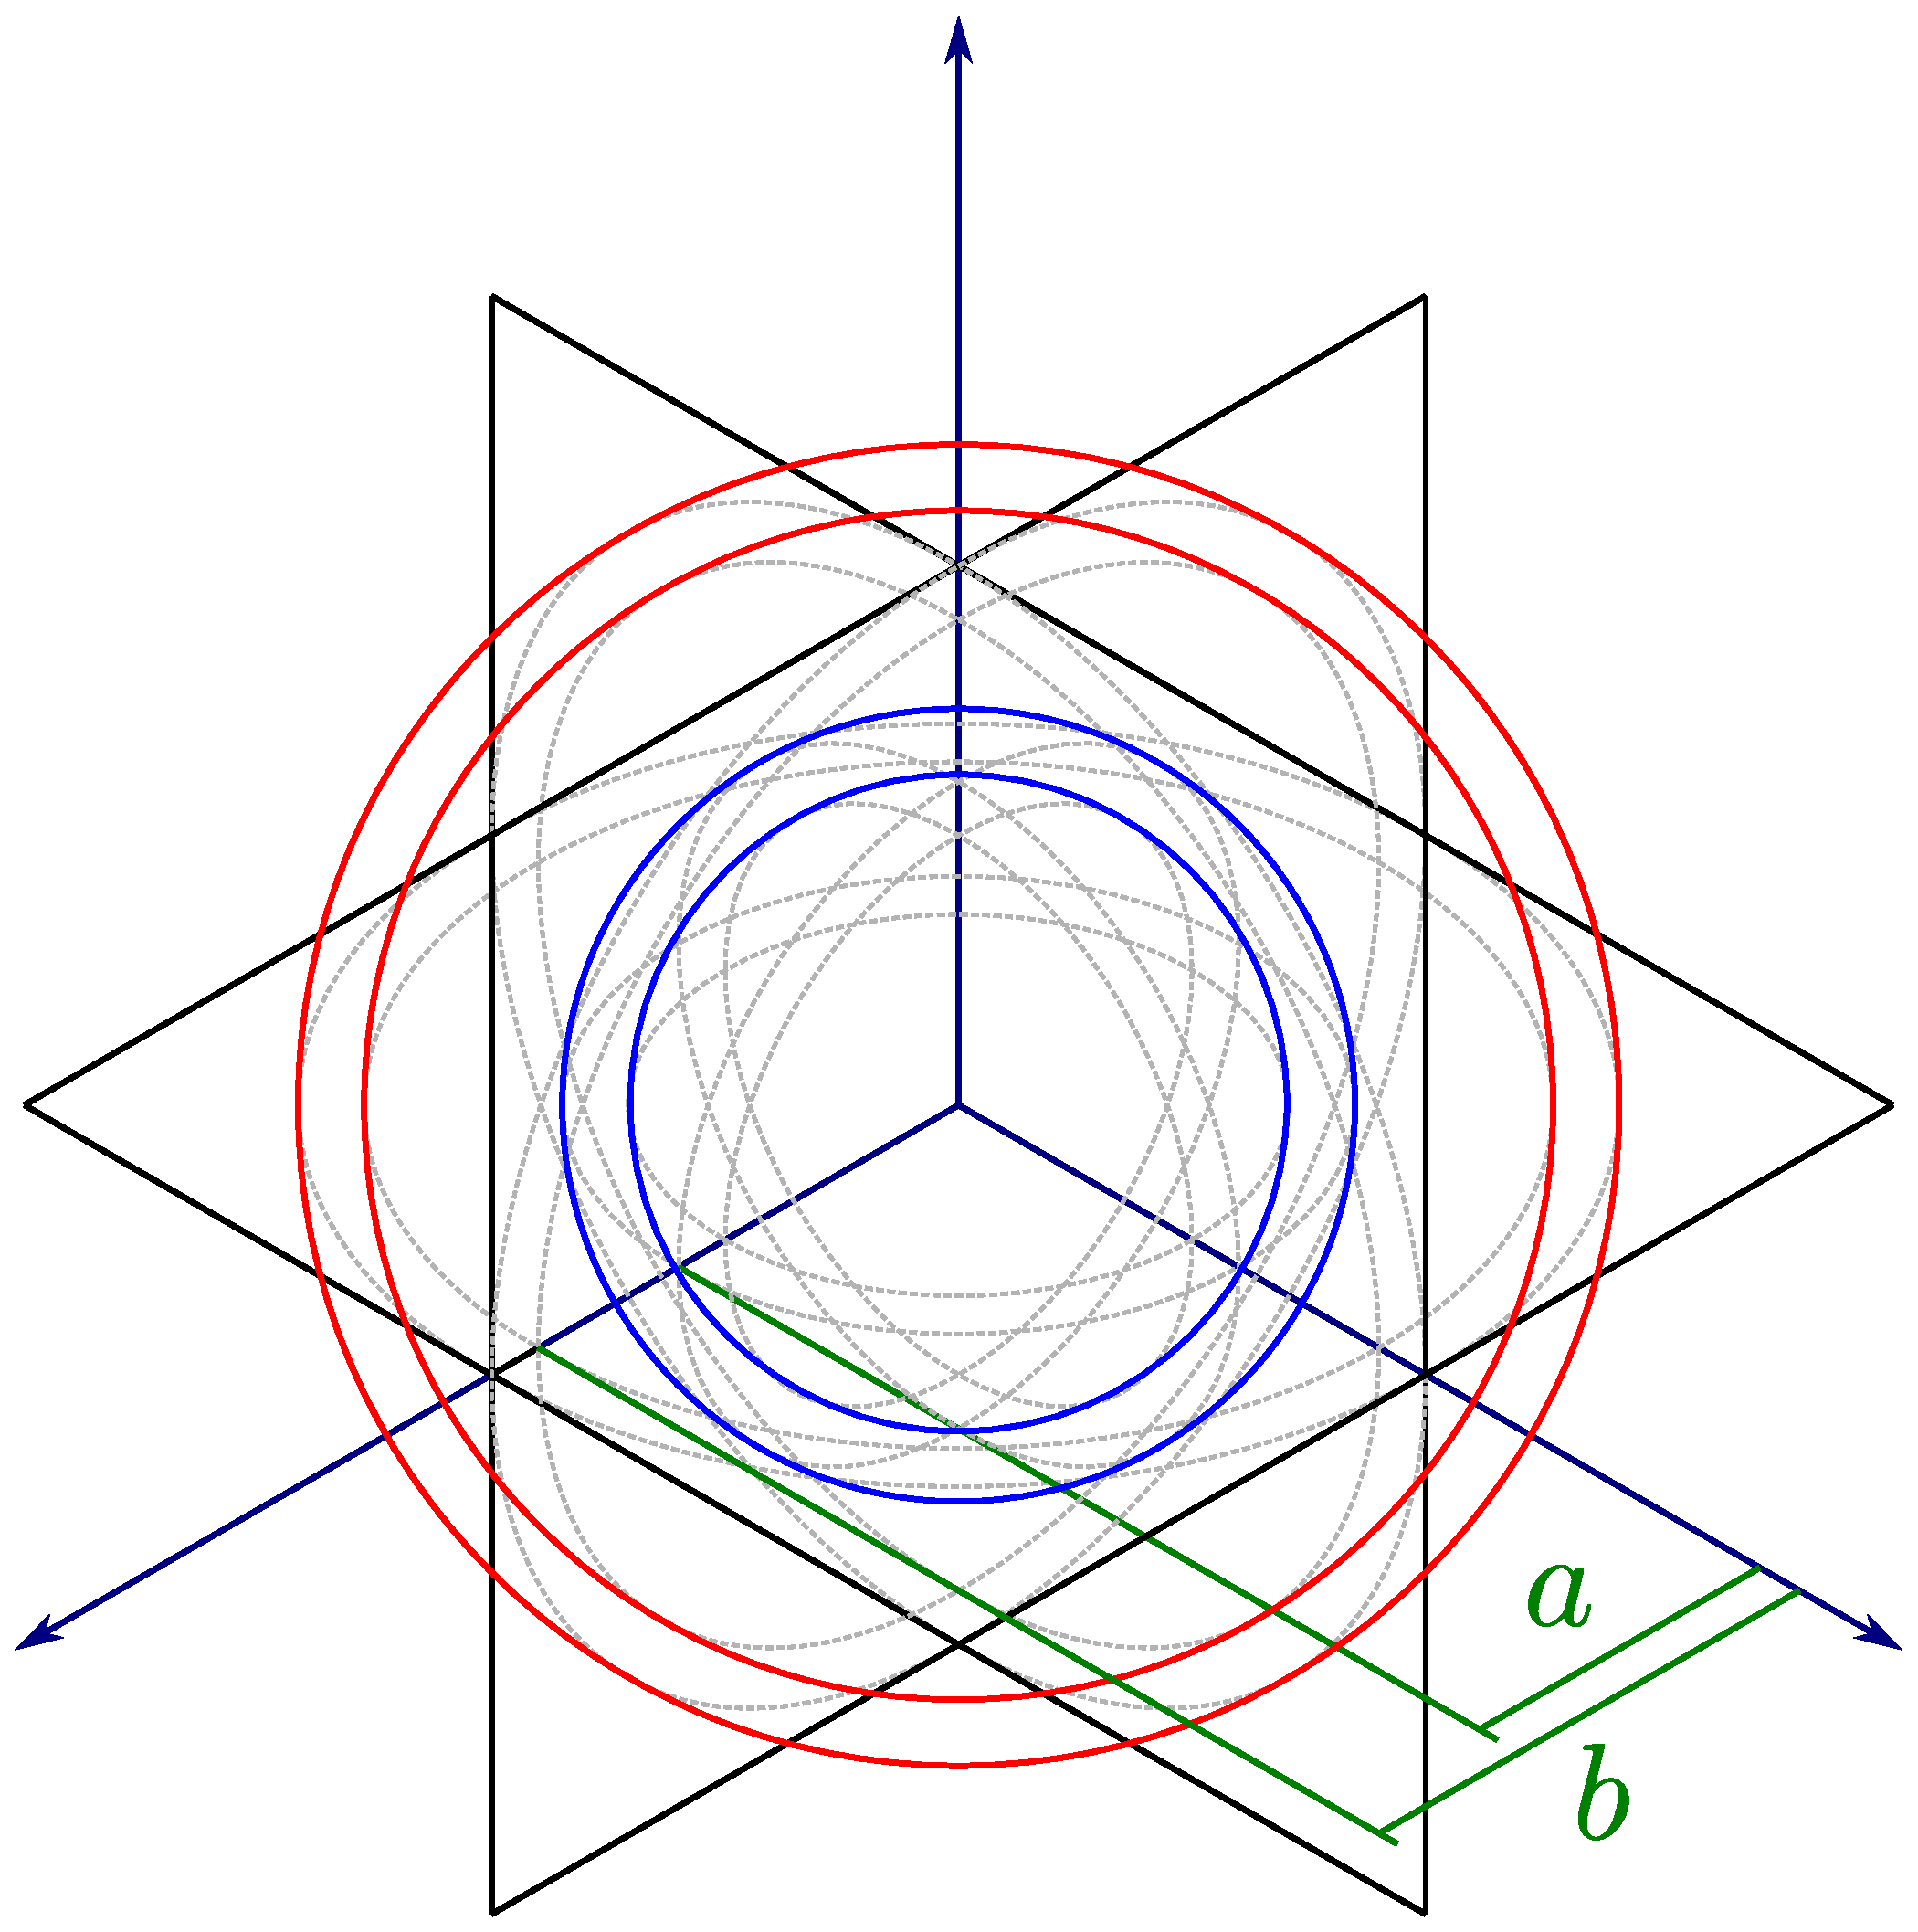
\includegraphics[scale=0.15]{resources/f2.eps}
\end{figure}
\vspace{0.20cm}

Usando una superficie \emph{gaussiana} sobre el capacitor para obtener el campo
eléctrico:

\begin{equation*}
    \oint\vec{E}\cdot d\vec{A}=\frac{Q_{enc}}{\epsilon_0}
\end{equation*}
\begin{equation*}
    E\,(2\pi r)(2r)=\frac{Q}{\epsilon_0}
\end{equation*}
\begin{equation*}
    E=\frac{Q}{\epsilon_0}\frac{1}{4\pi r^2}
     =\frac{Q}{4\pi\epsilon_0 r^2}
\end{equation*}
\begin{equation*}
    \vec{E}=\frac{Q}{4\pi\epsilon_0 r^2}\hat{u}_r
\end{equation*}
\vspace{0.5cm}

Calculando la diferencia de potencial eléctrico:

\begin{equation*}
    \hat{E}=-\nabla\varphi
\end{equation*}
\begin{equation*}
    \frac{Q}{4\pi\epsilon_0 r^2}\hat{u}_r=-\frac{d\varphi}{dr}\hat{u}_r
\end{equation*}
\begin{equation*}
    \frac{Q}{4\pi\epsilon_0 r^2}dr=-d\varphi
\end{equation*}
\begin{equation*}
    \frac{Q}{4\pi\epsilon_0}\int_a^b\frac{dr}{r^2}
    =-\int_{\varphi^+}^{\varphi^-}d\varphi
\end{equation*}
\begin{equation*}
    V=\frac{Q}{4\pi\epsilon_0}(-\frac{1}{r}\Biggr|_a^b)
     =\frac{Q}{4\pi\epsilon_0}\left(\frac{1}{a}-\frac{1}{b}\right)
\end{equation*}
\vspace{0.5cm}

Considerando la definición de capacitancia $Q=CV$:

\begin{equation*}
    C=\frac{Q}{V}
     =Q\,\frac{4\pi\epsilon_0}{Q\,\left(\frac{1}{a}-\frac{1}{b}\right)}
     =\frac{4\pi\epsilon_0}{\frac{1}{a}-\frac{1}{b}}
\end{equation*}

\end{document}

